\subsection{differentPlayerTypes}
\label{ss:differentPlayerTypes}
\FloatBarrier

\paragraph{Einleitung}
Dieses Package umfasst alle verschiedenen Spielertypen sowie die Klasse zum Instantiieren der Spielerreferenzen \lstref{fig:differentPlayerTypesPackage}. 

\begin{figure}
	\centering
	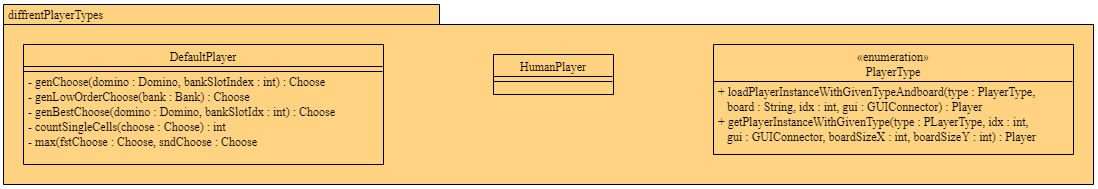
\includegraphics[width=\linewidth]{pics/differentPlayerTypesPackage}
	\caption{UML-Darstellung des differentPlayerTypes packages}
	\label{fig:differentPlayerTypesPackage}
\end{figure}

\import{programmierhandbuch/grundlegendeKlassen/differentPlayerTypes/defaultAIPlayer/}{defaultAIPlayerClassDoc.tex}
\import{programmierhandbuch/grundlegendeKlassen/differentPlayerTypes/humanPlayer/}{humanPlayerClassDoc.tex}
\import{programmierhandbuch/grundlegendeKlassen/differentPlayerTypes/playerType/}{playerTypeClassDoc.tex}